\documentclass[12pt,a4paper, margin=1in]{article}
\usepackage{fullpage}
\usepackage{amsfonts, amsmath, pifont}
\usepackage{amsthm}
\usepackage{graphicx}
\usepackage{tkz-euclide}
\usepackage{amsmath}
\usepackage{tikz}
\usepackage{amsmath}
\usepackage{pgfplots}
\usepackage{tikz}
\usepackage{geometry}
 \geometry{
 a4paper,
 total={210mm,297mm},
 left=10mm,
 right=10mm,
 top=5mm,
 bottom=10mm,
 }
 \author{
  Göçer, Anıl Eren\\
  \texttt{e2448397@ceng.metu.edu.tr}
}
\title{CENG 382 - Analysis of Dynamic Systems \\
20221\\
Take Home Exam 2 Solutions}
\begin{document}
\maketitle

\noindent\rule{19cm}{1.2pt}

\begin{enumerate}
% Write your solutions in the following items.

    \item % Q1
        \begin{enumerate}
            \item Markov chain can be modeled with the following diagram where 1 represents professionals,
            2 represents skilled laborers and 3 represents unskilled laborers. \\

\begin{center}
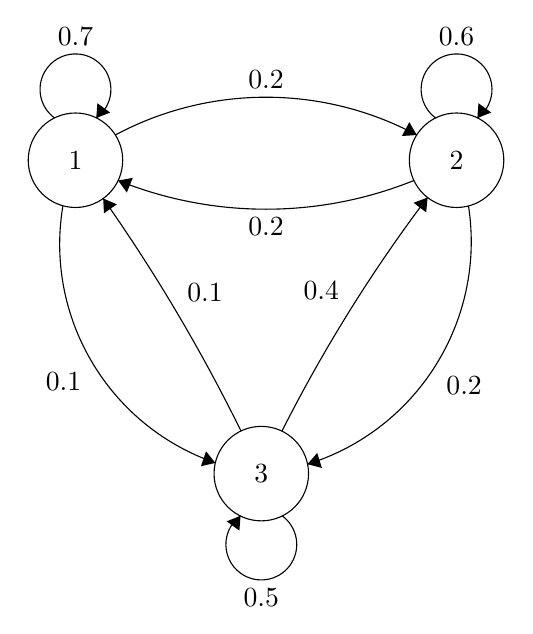
\begin{tikzpicture}[scale=0.2]
\tikzstyle{every node}+=[inner sep=0pt]
\draw [black] (28.1,-16.1) circle (3);
\draw (28.1,-16.1) node {$1$};
\draw [black] (39.9,-36) circle (3);
\draw (39.9,-36) node {$3$};
\draw [black] (52.3,-16.1) circle (3);
\draw (52.3,-16.1) node {$2$};
\draw [black] (26.777,-13.42) arc (234:-54:2.25);
\draw (28.1,-8.85) node [above] {$0.7$};
\fill [black] (29.42,-13.42) -- (30.3,-13.07) -- (29.49,-12.48);
\draw [black] (36.985,-35.315) arc (-109.07021:-189.59689:14.686);
\fill [black] (36.98,-35.32) -- (36.39,-34.58) -- (36.07,-35.53);
\draw (28.5,-30.18) node [left] {$0.1$};
\draw [black] (30.632,-14.495) arc (118.13388:61.86612:20.292);
\fill [black] (49.77,-14.5) -- (49.3,-13.68) -- (48.83,-14.56);
\draw (40.2,-11.6) node [above] {$0.2$};
\draw [black] (50.977,-13.42) arc (234:-54:2.25);
\draw (52.3,-8.85) node [above] {$0.6$};
\fill [black] (53.62,-13.42) -- (54.5,-13.07) -- (53.69,-12.48);
\draw [black] (49.592,-17.386) arc (-68.02263:-111.97737:25.095);
\fill [black] (30.81,-17.39) -- (31.36,-18.15) -- (31.74,-17.22);
\draw (40.2,-19.71) node [below] {$0.2$};
\draw [black] (53.056,-18.998) arc (8.81856:-72.67391:14.806);
\fill [black] (42.83,-35.4) -- (43.75,-35.64) -- (43.45,-34.69);
\draw (51.62,-30.39) node [right] {$0.2$};
\draw [black] (41.223,-38.68) arc (54:-234:2.25);
\draw (39.9,-43.25) node [below] {$0.5$};
\fill [black] (38.58,-38.68) -- (37.7,-39.03) -- (38.51,-39.62);
\draw [black] (29.859,-18.53) arc (35.13054:26.20236:110.239);
\fill [black] (29.86,-18.53) -- (29.91,-19.47) -- (30.73,-18.9);
\draw (35.17,-24.49) node [right] {$0.1$};
\draw [black] (41.211,-33.302) arc (153.20642:142.93823:97.67);
\fill [black] (50.46,-18.47) -- (49.57,-18.8) -- (50.37,-19.41);
\draw (44.87,-24.39) node [left] {$0.4$};
\end{tikzpicture}
\end{center}

The state transition matrix corresponding to this markov chain is found as:
            \begin{center}
                $A = \begin{bmatrix}
                    0.7 & 0.2 & 0.1 \\
                    0.2 & 0.6 & 0.2 \\
                    0.1 & 0.4 & 0.5 
            \end{bmatrix}$
            \end{center}

            \item  To find this probability, we need to find $A^2$ 

\begin{center}
$A^2 =
\begin{bmatrix}
0.7 & 0.2 & 0.1 \\
0.2 & 0.6 & 0.2 \\
0.1 & 0.4 & 0.5 
\end{bmatrix}.
\begin{bmatrix}
0.7 & 0.2 & 0.1 \\
0.2 & 0.6 & 0.2 \\
0.1 & 0.4 & 0.5 
\end{bmatrix} = 
\begin{bmatrix}
0.54 & 0.3 & 0.16 \\
0.28 & 0.48 & 0.24 \\
0.2 & 0.46 & 0.34 
\end{bmatrix}
$ 
\end{center}

The entry $a_{31}$ of this matrix, which is 0.2, gives the probability asked in the question. \\\\
\textbf{Answer: } 0.2

\newpage
            \item Again, in order to find this probability, we need to find $A^2$.
\begin{center}
$A^2 =
\begin{bmatrix}
0.7 & 0.2 & 0.1 \\
0.2 & 0.6 & 0.2 \\
0.1 & 0.4 & 0.5 
\end{bmatrix}.
\begin{bmatrix}
0.7 & 0.2 & 0.1 \\
0.2 & 0.6 & 0.2 \\
0.1 & 0.4 & 0.5 
\end{bmatrix} = 
\begin{bmatrix}
0.54 & 0.3 & 0.16 \\
0.28 & 0.48 & 0.24 \\
0.2 & 0.46 & 0.34 
\end{bmatrix}
$ 
\end{center}

The entry $a_{11}$ of this matrix, which is $0.54$, gives the probability asked in the question. \\\\
\textbf{Answer: } 0.54


            \item First we need to find the transpose of $A$:
\begin{center}
$A^T=
\begin{bmatrix}
0.7 & 0.2 & 0.1 \\
0.2 & 0.6 & 0.4 \\
0.1 & 0.2 & 0.5
\end{bmatrix}
$ 
\end{center}

We know that $\lambda = 1$ is eigenvalue of stochastic matrices. We need to compute corresponding eigenvector such that $A^T . $ $ v = v$: 

\begin{center}
$
\begin{bmatrix}
0.7 & 0.2 & 0.1 \\
0.2 & 0.6 & 0.4 \\
0.1 & 0.2 & 0.5
\end{bmatrix}
 . 
\begin{bmatrix}
    v_1 \\
    v_2 \\
    v_3
\end{bmatrix} = 
\begin{bmatrix}
    v_1 \\
    v_2 \\
    v_3
\end{bmatrix}$ 
\end{center}
This gives the equations:

\begin{center}
\begin{equation*} \label{eq1}
\begin{split}
        0.7 v_1 + 0.2 v_2 + 0.1 v_3 & = v_1 \\
        0.2 v_1 + 0.6 v_2 + 0.4 v_3 & = v_2 \\
        0.1 v_1 + 0.2 v_2 + 0.5 v_3 & = v_3 
\end{split}
\end{equation*}    
\end{center}

From there, we found $v_1 = \dfrac{6}{17}, v_2 = \dfrac{7}{17}, v_3= \dfrac{4}{17}.$  \\ \\
So, we compute the eigenvector $v$ as 
$v = \begin{bmatrix}
    6 / 17 \\
    7 / 17 \\
    4 / 17
\end{bmatrix}
$ . \\\\
Hence, long term behavior of the matrix A, representing the markov chain, can be computed by replacing the rows of the matrix with transpose of the eigenvector $v^T$. 

\begin{center}
$A^{100} = A^{\infty} = 
\begin{bmatrix}
6/17 & 7/17 & 4/17 \\
6/17 & 7/17 & 4/17 \\
6/17 & 7/17 & 4/17 \\
\end{bmatrix} = 
\begin{bmatrix}
0.352941 & 0.411765 & 0.235294 \\
0.352941 & 0.411765 & 0.235294 \\ 
0.352941 & 0.411765 & 0.235294
\end{bmatrix}
$ 
\end{center}
The behavior of the markov chain after $100^{th}$ generation can be summarized by the following: \\ \\
$100^{th}$ generation son of a person of any type is professional with the probability $0.352941$, skilled laborer with the probability $0.411765$ and unskilled laborer with the probability $0.235294$. 
        \end{enumerate}

\newpage
        
    \item % Q2
        \begin{enumerate}
            \item In order to show that the system is controllable, we need to check controllability matrix M, if M has rank n (equal to number of rows and columns). If that's the case , the system is controllable. \

Let's calculate M;
\begin{center}
    M = \begin{bmatrix}
        B & AB & A^2B
    \end{bmatrix}
\end{center}

We know that;
\begin{center}
    A = \begin{bmatrix}
        0 & 0 & 1 \\
        -2 & 0 & -1 \\
        0 & 1 & 0
    \end{bmatrix},
    \space 
    B =  \begin{bmatrix}
        1 & 0 & 0
    \end{bmatrix}
\end{center}

So, we find M as;
\begin{center}
    M = \begin{bmatrix}
       1 & 0 & 0 \\
       0 & -2 & 0 \\
       0 & 0 & -2
    \end{bmatrix}
\end{center}

We see that $M$ has 3 linearly independent rows, so it has rank $n = 3$. \\ This means that the sytem is \textbf{controllable}.

            \item We have $
            x(0) = \begin{bmatrix}
       1 \\ 1 \\ 1 
    \end{bmatrix}
            $ and $
            x(3) = \begin{bmatrix}
       4 \\ 4 \\ 4
    \end{bmatrix}
            $.

\begin{center}
    $x(1) = Ax(0) + Bu(0) = \begin{bmatrix}
        0 & 0 & 1 \\
        -2 & 0 & -1 \\
        0 & 1 & 0
    \end{bmatrix}.\begin{bmatrix}
       1 \\ 1 \\ 1 
    \end{bmatrix} + \begin{bmatrix}
       u(0)  \\ 0 \\ 0 
    \end{bmatrix} = \begin{bmatrix}
       u(0) +  1 \\ -3 \\ 1 
    \end{bmatrix}$
\end{center}
\begin{center}
    $x(2) =  Ax(1) + Bu(1) =
\begin{bmatrix}
        0 & 0 & 1 \\
        -2 & 0 & -1 \\
        0 & 1 & 0
    \end{bmatrix}.
\begin{bmatrix}
       u(0) +  1 \\ -3 \\ 1 
    \end{bmatrix} + \begin{bmatrix}
       u(1)  \\ 0 \\ 0 
    \end{bmatrix} = 
\begin{bmatrix}
       u(1) +  1 \\ -2u(0)-3 \\ -3 
    \end{bmatrix}
    $ 
\end{center}

\begin{center}
    $x(3) = Ax(2) + Bu(2) = 
 \begin{bmatrix}
        0 & 0 & 1 \\
        -2 & 0 & -1 \\
        0 & 1 & 0
    \end{bmatrix}.\begin{bmatrix}
       u(1) +  1 \\ -2u(0)-3 \\ -3 
    \end{bmatrix} + \begin{bmatrix}
       u(2)  \\ 0 \\ 0
    \end{bmatrix} = \begin{bmatrix}
       u(2) - 3  \\ -2u(1) + 1 \\ -2u(0) - 3 
    \end{bmatrix}$
\end{center}
It follows as:
\begin{center}
    $x(3) = \begin{bmatrix}
       4 \\ 4 \\ 4
    \end{bmatrix} = \begin{bmatrix}
       u(2) - 3  \\ -2u(1) + 1 \\ -2u(0) - 3 
    \end{bmatrix}$
\end{center}
From there,  we find $u(0) = -7/2, u(1) = -3/2 $ and $ u(2) = 7$. \\ \\
This sequence of inputs leads to system to the given point $\begin{bmatrix}
       4 \\ 4 \\ 4
    \end{bmatrix}$ in exactly 3 steps. 
        \end{enumerate}
\begin{center}
     $\begin{bmatrix}
       u(0) \\ u(1) \\ u(2)
    \end{bmatrix} = \begin{bmatrix}
       -7/2 \\ -3\2 \\ 7 
    \end{bmatrix}$
\end{center}

        
\newpage

    \item % Q3
        \begin{enumerate}
            \item 
            \item 
        \end{enumerate}
        
        
    \item % Q4 
        \begin{enumerate}
            \item 
            \item 
        \end{enumerate}


\end{enumerate}

\end{document}
